\documentclass[crop,tikz]{standalone}% 'crop' is the default for v1.0, before it was 'preview'
%\usetikzlibrary{...}% tikz package already loaded by 'tikz' option
% \usetikzlibrary{calc, backgrounds}
\usepackage{amsmath}
\newcommand{\bo}[1]{\boldsymbol{#1}}

\begin{document}
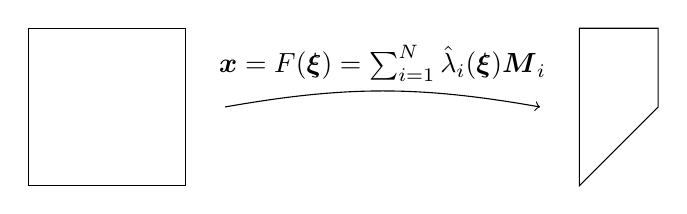
\begin{tikzpicture}
    % Globals
    \pgfmathsetmacro{\refXMin}{0}
    \pgfmathsetmacro{\refXMax}{2}
    \pgfmathsetmacro{\arrowWidth}{4}
    \pgfmathsetmacro{\arrowMarginX}{0.5}

    \coordinate (REF_SW) at (\refXMin, \refXMin);
    \coordinate (REF_NE) at (\refXMax, \refXMax);
    \pgfmathsetmacro{\x}{\refXMax+\arrowMarginX}
    \pgfmathsetmacro{\y}{(\refXMax-\refXMin)/2}
    \coordinate (LINE_W) at (\x, \y);
    \pgfmathsetmacro{\x}{\x+\arrowWidth}
    \coordinate (LINE_E) at (\x, \y);

    \draw[color=black] (REF_SW) rectangle (REF_NE);

    \draw[->] (LINE_W) to[out=10,in=170] node[midway, above]{
        $\bo{x} = F(\bo{\xi}) = \sum_{i=1}^N \hat{\lambda}_i(\bo{\xi})\bo{M}_i$
        % $\begin{pmatrix}x \\ y\end{pmatrix} = F(\xi, \eta) = \sum_{i=1}^N \hat{\lambda}(\xi, \eta)M_i$
    } (LINE_E);

    \pgfmathsetmacro{\x}{\refXMax + 2*\arrowMarginX + \arrowWidth};
    \draw (\x, 0) to ++(1,1) to ++(0, 1) to ++(-1,0) to cycle;


\end{tikzpicture}
\end{document}